\subsection{SOM Architecture and Initialization Sensitivity}
\label{sec:som_sensitivity}

A sensitivity study was performed to determine how the SOM representation
depends on lattice architecture and random initialization. Four square
architectures were evaluated: \(3\times3\), \(4\times4\), \(5\times5\),
and \(6\times6\), corresponding to 9, 16, 25, and 36 neurons,
respectively.

For each architecture, five independent initializations were evaluated using
random seeds 1, 11, 21, 31, and 42, giving a total of 20 SOM training runs.
The M40 CFD solution, input features, feature standardization, SOM training
algorithm, and 20000 training iterations were held fixed across all runs.
The initial neighborhood width was also kept fixed at
\(\sigma_0=2\). Consequently, its size relative to the SOM lattice changes
with architecture; this choice was retained deliberately so that the tested
configurations differed only in lattice size and random initialization under
the common training specification.

The sensitivity analysis considered several complementary quantities:
quantization error, SOM-interface fraction, partition stability between
random initializations, and spatial stability of the 40 highest-priority
interface seeds. These metrics characterize different properties of the SOM
and should not individually be interpreted as measures of adaptive-mesh
accuracy.

Table~\ref{tab:som_architecture_sensitivity} summarizes the architecture-level
statistics obtained by averaging over the five random initializations.

\begin{table}[htbp]
\centering
\caption{Sensitivity of the SOM representation to lattice architecture.
Reported values are averages over five random seeds.}
\label{tab:som_architecture_sensitivity}
\begin{tabular}{cccccc}
\hline
Architecture & Neurons & Mean QE & SD QE & Interface fraction & Occupied neurons \\
\hline
\(3\times3\) & 9  & 0.6468 & 0.0136 & 0.3078 & 9.0 \\
\(4\times4\) & 16 & 0.5049 & 0.0166 & 0.4381 & 16.0 \\
\(5\times5\) & 25 & 0.4023 & 0.0036 & 0.5478 & 25.0 \\
\(6\times6\) & 36 & 0.3431 & 0.0037 & 0.6304 & 35.8 \\
\hline
\end{tabular}
\end{table}

Increasing the number of SOM neurons systematically reduced the mean
quantization error for the tested configurations. The mean QE decreased from
approximately 0.647 for the \(3\times3\) architecture to 0.343 for the
\(6\times6\) architecture. This behavior is expected because a larger number
of prototypes provides greater representational capacity in the standardized
feature space.

At the same time, the fraction of M40 cells classified as SOM-interface cells
increased substantially, from approximately 30.8\% for \(3\times3\) to
43.8\% for \(4\times4\), 54.8\% for \(5\times5\), and 63.0\% for
\(6\times6\). Thus, increasing SOM resolution produces a finer partition of
the CFD state space but also generates a progressively denser spatial
interface network.

The reduction in quantization error should therefore not be interpreted as
evidence that the larger SOM architectures are automatically preferable for
adaptive refinement. Quantization error measures representation in feature
space, whereas the usefulness of a SOM-derived refinement criterion depends
on how the resulting state partition and interfaces contribute to subsequent
mesh-refinement decisions.

\subsubsection{Partition stability across random initializations}

Because SOM training depends on initialization, the stability of the learned
cell partition was evaluated across the five random seeds. Direct comparison
of BMU labels is not sufficient because neuron labels can be permuted between
independent SOM trainings. Partition similarity was therefore evaluated using
the Adjusted Rand Index (ARI) and a same-cluster pairwise Jaccard measure.

\begin{table}[htbp]
\centering
\caption{Stability of the SOM partition across random initializations.
Statistics are calculated from pairwise comparisons between the five seeds
for each architecture.}
\label{tab:som_partition_stability}
\begin{tabular}{ccccc}
\hline
Architecture & Mean ARI & SD ARI & Mean pair Jaccard & SD pair Jaccard \\
\hline
\(3\times3\) & 0.901 & 0.021 & 0.847 & 0.029 \\
\(4\times4\) & 0.771 & 0.031 & 0.656 & 0.038 \\
\(5\times5\) & 0.795 & 0.043 & 0.679 & 0.058 \\
\(6\times6\) & 0.674 & 0.051 & 0.526 & 0.056 \\
\hline
\end{tabular}
\end{table}

The \(3\times3\) architecture produced the most stable partition among the
tested configurations, with a mean ARI of approximately 0.901. The
\(6\times6\) architecture produced the lowest mean ARI, approximately 0.674.
The behavior was not strictly monotonic with lattice size: the \(5\times5\)
architecture was somewhat more stable than the \(4\times4\) architecture
according to both partition metrics.

These results show that the reduction in quantization error obtained with
larger maps does not imply increased robustness to random initialization.
In particular, the \(6\times6\) configuration achieved the lowest mean
quantization error while also exhibiting the lowest partition stability of
the four architectures tested. Architecture selection therefore involves
more than minimizing quantization error alone.

\subsubsection{Spatial stability of high-priority interface seeds}

Partition stability does not by itself determine whether the cells considered
most important for refinement move to completely different physical regions.
The spatial stability of the 40 highest-priority SOM-interface seeds was
therefore evaluated separately.

\begin{table}[htbp]
\centering
\caption{Spatial stability of the 40 highest-priority SOM-interface seeds
across random initializations.}
\label{tab:som_spatial_stability}
\begin{tabular}{ccccc}
\hline
Architecture & Exact Jaccard & Exact match & \(r=1\) match & \(r=2\) match \\
\hline
\(3\times3\) & 0.698 & 0.820 & 0.955 & 0.986 \\
\(4\times4\) & 0.507 & 0.665 & 0.895 & 0.960 \\
\(5\times5\) & 0.551 & 0.708 & 0.931 & 0.970 \\
\(6\times6\) & 0.609 & 0.753 & 0.951 & 0.988 \\
\hline
\end{tabular}
\end{table}

Exact agreement between the Top-40 seed sets varied appreciably with random
initialization. For the \(4\times4\) architecture used in the main study,
the mean exact Jaccard similarity was approximately 0.507 and the mean exact
cell-match fraction was 0.665.

However, much of this variation was spatially local. When a selected cell
was considered matched if a corresponding selection occurred within one
M40 cell layer, the mean match fraction for the \(4\times4\) architecture
increased to approximately 0.895. With a two-cell-layer tolerance it
increased to approximately 0.960. Similar behavior was observed for the
other tested architectures.

These proximity statistics indicate that different initializations often
identify nearby regions even when they do not select exactly the same cells.
They should nevertheless be interpreted cautiously: the proximity measure
allows local many-to-one correspondence and is not equivalent to the overlap
of the final refined regions or to equality of the resulting adaptive CFD
solutions.

Figure~\ref{fig:som_sensitivity_consensus} provides a spatial view of these
sensitivity results. The upper row shows how frequently each M40 cell was
classified as a SOM-interface cell across the five random initializations,
whereas the lower row shows the corresponding selection frequency among the
40 highest-priority interface seeds.

\begin{figure}[htbp]
\centering
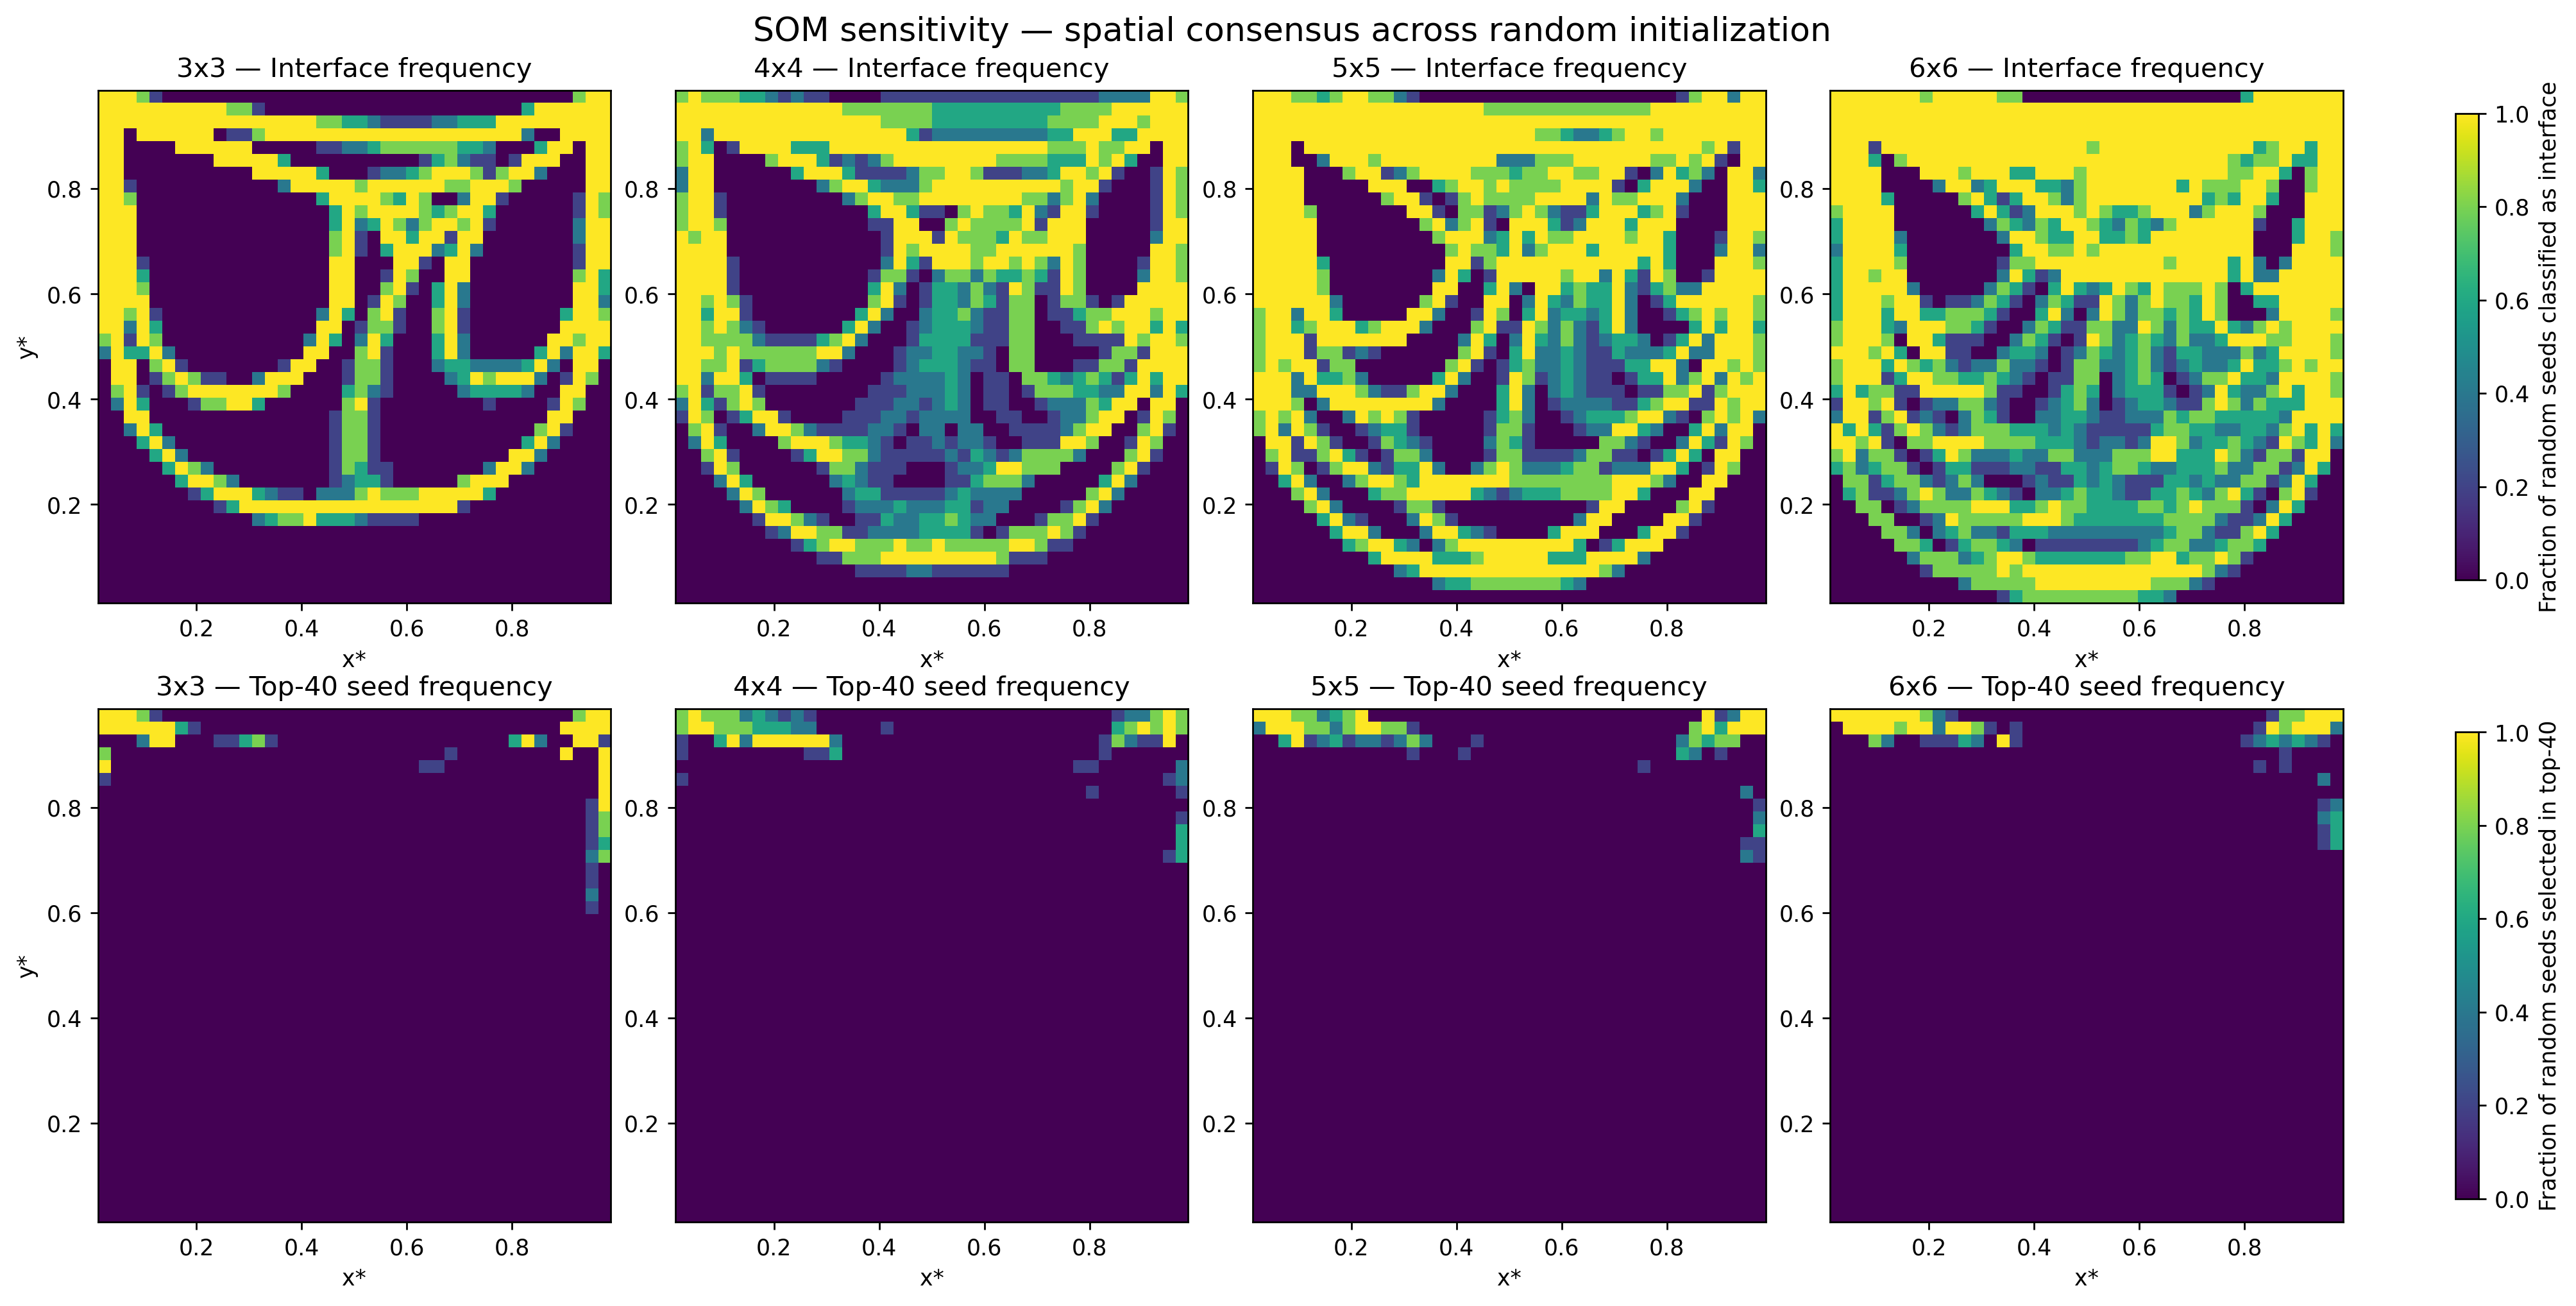
\includegraphics[width=0.98\textwidth]
{figures/som_sensitivity_consensus.png}
\caption{Spatial consensus across five random initializations for the
\(3\times3\), \(4\times4\), \(5\times5\), and \(6\times6\) SOM
architectures. The upper row shows SOM-interface frequency and the lower row
shows Top-40 seed-selection frequency.}
\label{fig:som_sensitivity_consensus}
\end{figure}

The consensus maps reinforce the quantitative results. Increasing the SOM
size produces a denser network of state interfaces, while the highest-priority
interface selections remain concentrated within comparatively localized
regions of the cavity. Differences between random initializations therefore
affect the exact partition and exact selected cells without necessarily
relocating all high-priority selections to unrelated physical regions.

The sensitivity study does not identify a uniquely optimal SOM architecture.
The \(3\times3\) map provides the highest partition stability but the
coarsest representation among the tested configurations. Conversely, the
\(6\times6\) map provides the lowest mean quantization error but generates
the densest interface network and exhibits the lowest mean partition
stability. The \(4\times4\) configuration used in the main adaptive study
should therefore be interpreted as the nominal architecture investigated in
that study, rather than as an architecture demonstrated to be optimal.

More generally, the results demonstrate that SOM architecture and random
initialization constitute relevant modeling choices for the proposed
interface-based refinement framework. Robustness of a fixed-seed result
should not be conflated with robustness to alternative initializations, and
future applications should evaluate architecture and initialization
sensitivity for the flow problem under consideration.
